\subsection{Knee Joint and ACL} 
As the paper includes interdisciplinary content, it is necessary to first provide information in this section about the mechanical properties of the knee used throughout the paper. The knee joint is the largest joint in the human body that connects the femur and tibia. ACL is one of the four major ligaments in the knee. It originates from deep within the lower extremity of the femur and attaches in front of the spine of tibia. The Figure~\ref{fig:knee_anatomy} below is representative of the knee anatomy and the location of ACL. 

\begin{figure}[h]
  \begin{center}
    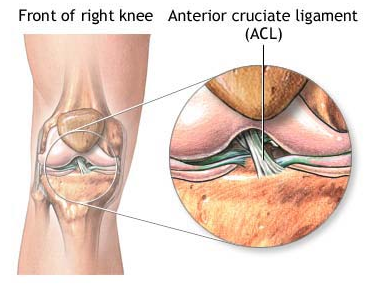
\includegraphics[width=3in]{images/acl_anatomy.bmp}
  \end{center}
  \caption{Knee anatomy and location of ACL}
  \label{fig:knee_anatomy}
\end{figure}

\subsection{Knee Flexion Angles}
ACL is responsible for resisting anterior translation and medial rotation of the tibia, in relation to the femur. This resistance is crucial for controlling the forward movement and twisting of the knee. Major cause of ACL injury is small knee flexion angle along with medial rotation. The knee flexion angle is the angle between the femur and the tibia. The medial rotation is the internal rotation of the knee towards the midline axis of the human body. As a result, these angles are an important indicator for the injury.

\subsection{Asymmetric distributed forces}
Another common reason for the ACL injury is due to asymmetric distributed forces acting on the joint. As these forces are not equally distributed, the resultant force direction does not pass through the vertical axis at the center of the leg. This resultant force causes anterior translation and medial rotation. Once the forces exceed the resistance offered by the ACL,  the ACL ruptures due to excessive strain (TODO cite GRIFFIN et al). Now, these forces are caused due to sudden movements such as changing directions or landing from a jump, which are most common in sports (TODO cite GRIFFIN et al). These decelerations generally happen as fast as 50ms (TODO cite some paper), and therefore, ekwip needs to be able to measure the deceleration as fast as 10s of milliseconds. The decelerations can then be related to the forces to provide a more complete analysis for risk calculations.